\documentclass{article}
\documentclass[12pt,oneside,reqno]{amsart}
\usepackage{graphicx}
\usepackage{fullpage}
\usepackage{float}
\graphicspath{ {images/} }
\usepackage{titling}
\begin{document}
\pretitle{%
\begin{center}\LARGE
\rule{5in}{1pt}\par
}
\posttitle{\par\rule{5in}{0.5pt}\end{center}\vskip 0.5em}

 \title{\\\Huge \bfseries ECEN 325
\\ \LARGE Final Project
\\ \large -- CMOS Amplifier --\\}

\author{Caleb Clark\\Dariusz Mrugala}
\date{December 11th, 2017}
\maketitle
\thispagestyle{empty}
\clearpage
\thispagestyle{empty}
\tableofcontents
\setlength\parindent{0pt}
\pagebreak
\setcounter{page}{1}
\section{Introduction \& Objectives}
\subsection{Overview}
 \quad \quad This project involves the design and testing of a CMOS amplifier. This amplifier will utilize multiple stages and configurations. A high-level design of this amplifier can be seen below (Figure 1).   \\
	\begin{figure}[H]
    	\centerline{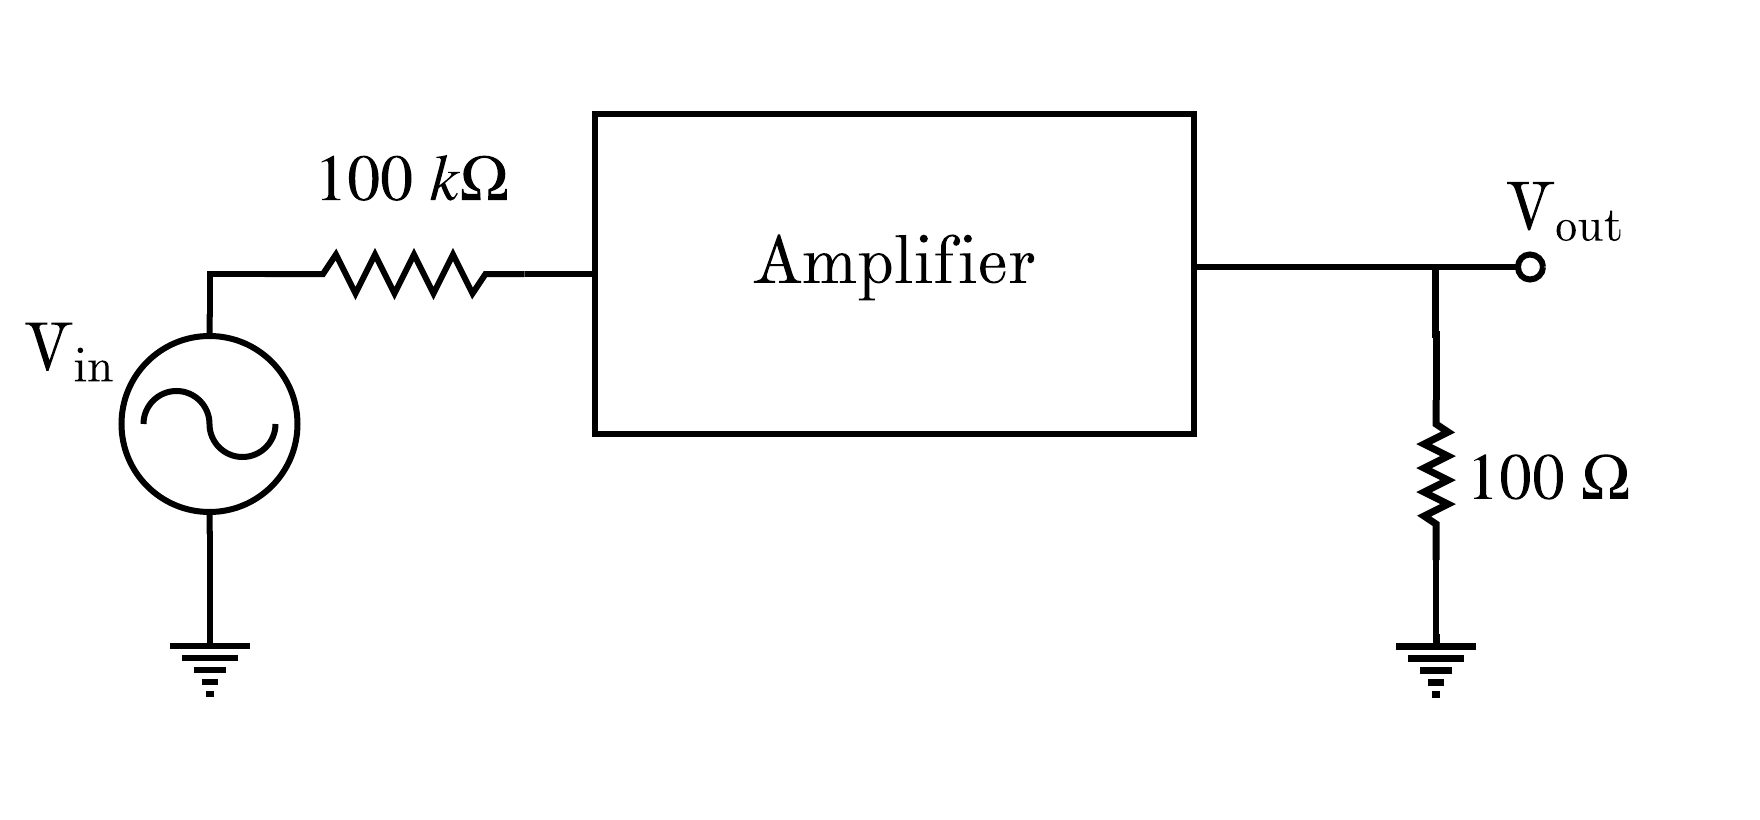
\includegraphics[width=0.75\textwidth]{high_level}}
    	\caption{\textbf{High-level Design}}
    \end{figure}
    
\subsection{Requirements}
\quad \quad The amplifier must meet the following requirements

\begin{itemize}
    \item $V_{DD}\ =\ 10 V$ 
    \item $R_{in}\ >\ 1\ M\Omega$
    \item $|A_v|\ =\ 40\ V/V$
    \item Load Resistance of 100 $\Omega$
    \item AC Coupled Input and Output
    \item Insensitive to temperature and $V_t$ variations
    \item Output voltage swing of 4 $V_{pp}$
    \item Discrete Components only
    \item Use either the CD4007 or 2N7000
    \item Low frequency -3 dB corner should be below 50 Hz
    \item High frequency -3 dB corner should be beyond 20 KHz
\end{itemize}
\pagebreak
\section{Design}
\quad \quad When designing an amplifier, there are many parameters that must be controlled for. It is important to keep all requirements in mind throughout the design process and not sacrifice one characteristic for another. In this section, the process of designing and refining the amplifier will be described in detail.
    \subsection{Assumptions}
    It is assumed that, for any transistors used, $\lambda = 0$ and therefore $r_0 = \infty.$ It is also assumed that when the AC input's frequency is zero, the capacitors in the circuit act as open circuits and when the frequency is very large, the capacitor behaves as an AC short. 
    \subsection{Procedure}
  \par
  \quad \quad When deciding on a general setup, the first step was to choose the number of stages that was needed in order to meet the requirements. While it may be possible to achieve the requirements with two stages, it would be less than ideal to do this. In order to do this, the drain voltage, $V_D$, would need to be rather large. This would push the NMOS far into the saturation region and may cause increased distortion on the output signal. The downside of adding a stage is that there is a risk of decreasing the bandwidth by increasing the capacitance from the decoupling capacitors and parasitic capacitance in the transistors themselves. \\
  \par
  \quad Ultimately, the decision was made to design the amplifier with three stages. This would allow for the voltage gain to be split up over two stages and leave the final stage for buffering. The first stage will provide a gain a $\pm$ 8 V/V and the second will provide a gain of $\pm$ 6 V/V. The last stage will attenuate the signal by a factor $0.8\overline{333}$ to bring the gain from 48 V/V to 40 V/V. \\
  \par 
  \quad As mentioned above, the final stage will act as a buffer for the output signal. This means that, in addition to lowering the voltage gain, this stage needs to zero out any DC offset value that the signal has.  \\
  \par 
  \quad These three stages will be joined together with decoupling capacitors. These capacitors block the DC voltage and current and allow the subsequent stages to be properly biased. At first, these capacitors will all be set to the same value. During the refining process, these capacitors will be tuned in order to satisfy the requirements on the -3 dB corner frequencies.  \\
    \par
    \quad Another consideration to be made was which transistor to use. The 2N7000 was used because the transistor could sustain higher channel currents and more information was available on this transistor on the simulator software used (NI Multisim). This transistor also has a rather large threshold voltage (2 V). This helps design the amplifier to be insensitive to changes in threshold voltage. \\
    \par 
    \quad Finally, it is important to use components that are realistic in value. For example, it could be advantageous to use very large capacitors in the design. However, it would not be reasonable to use a 1 farad capacitor. \\
    \subsubsection{Design of the First Stage}
    When designing the first stage, there were some important considerations to be made. A configuration was needed that could provide a high gain and a high input impedance. The first stage also needed to account for the resistance of the sensor or microphone. A logical choice was the common-source stage with a bypass capacitor. This configuration can be seen in Figure 2 below.
    \begin{figure}[H]
    	\caption{\textbf{First Stage - Common-Source with Biasing}}
    	\centerline{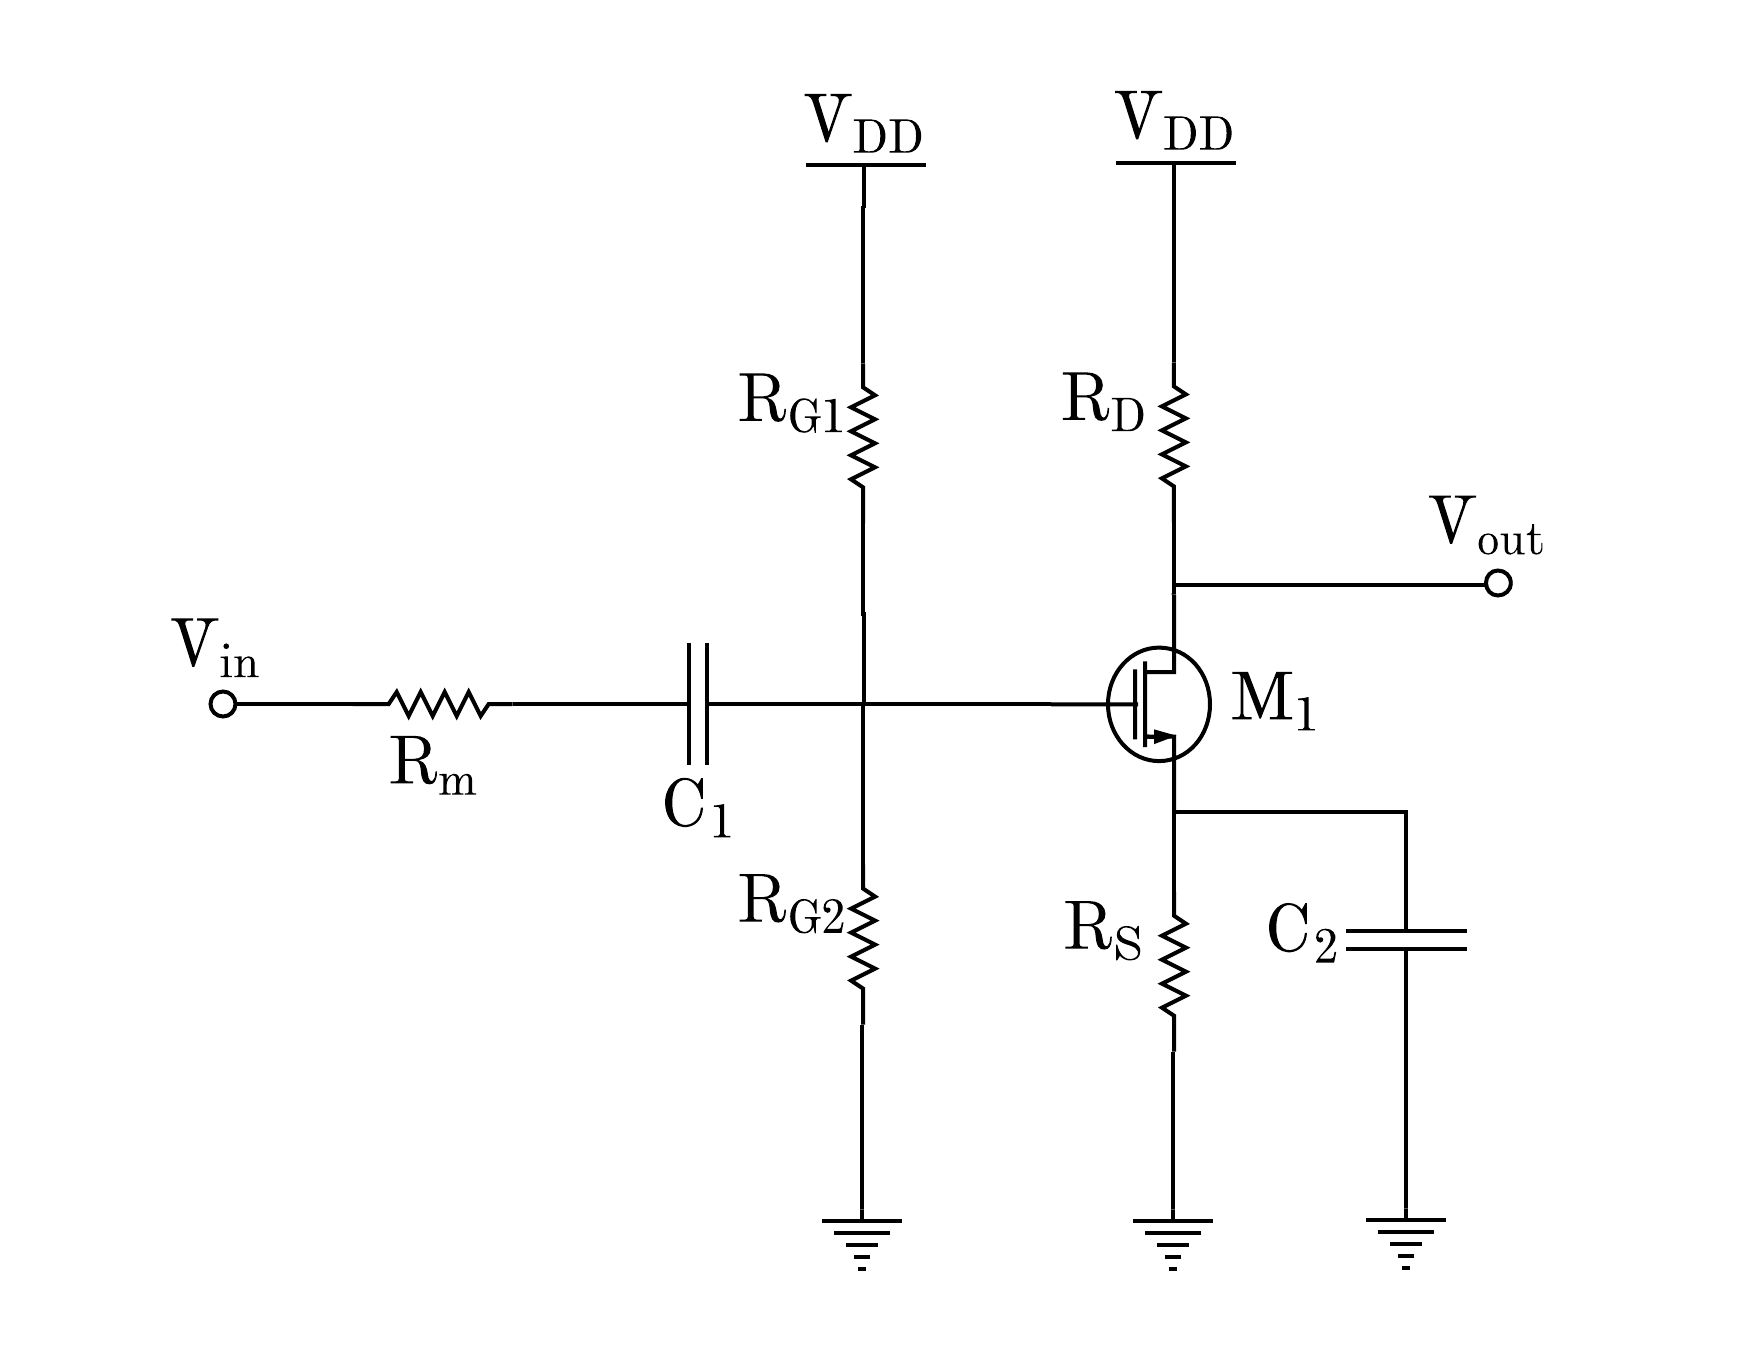
\includegraphics[width=0.75\textwidth]{first_stage}}
  
    \end{figure}
    \noindent The input impedance of this stage (and thereby the amplifier) is given by the following.
    $$ R_{in}\ =\ R_{G1}||R_{G2} $$
    The value of $R_{in}$ was chosen as 1.1 M$\Omega$ to satisfy the requirements that $R_{in}\ >\ 1\ M\Omega$. As mentioned above, the first stage was to provide a gain of $\pm$ 8 V/V. The gain of this configuration can be written as: \\
    $$ A_v\ =\ -\frac{R_{in}}{R_m\ +\ R_{in}}\ g_mR_D $$
    Since we decided that $R_{in}\ =\ 1.1M\Omega$ and $R_m$ is given as $100\ k\Omega$, an initial guess of $R_D\ =\ 100\ \Omega$ is made to obtain a value for the transconductance. Solving the equation above for $g_m$ and substituting the known values, $g_m$ is determined to be 0.0816 $\Omega^{-1}$. The value of the transconductance can also be represented by the following equation: 
    $$ g_m\ =\ \sqrt{2\beta I_D} $$
    Finding the channel current, $I_D$, will allow us to obtain the source resistor's value. First, though, the value of $\beta$ is needed. Examining the spice netlist for the 2N7000, the following specifications can be found.
    $$ W\ =\ 20\ mm,\ L\ =\ 2\ \mu m,\ \mu_n C_{ox}\ =\ 20\ \frac{mA}{V^2}$$
    Using this, the value of $\beta$ is computed to be 0.100783 $\frac{A}{V^2}$. Using this value of $\beta$ and the equation above, $I_D$ is found to be 33.03 mA. This value is tolerable by the transistor and will not exceed a standard resistor's power ratings. \\ 
    \par
    \quad With the value of $I_D$ obtained, the value of the source resistor can be obtained by choosing a value for the voltage $V_S$. We choose 400 mV for $V_S$ and compute $R_S$ to be $\approx\ 12.11\ \Omega$ with Ohm's law. The last things to obtain are the values of the individual biasing resistor values $R_{G1}$ and $R_{G2}$. To do this, the value of $V_{G}$ needs to be computed. This can be done by computing $V_{GS}$ and adding the value of $V_S$, which is 400 mV. $V_{GS}$ is computed by solving the following equation for $V_{GS}$.
    $$ g_m\ =\ \frac{2I_D}{V_{GS}\ -\ V_t} $$ 
    We find that $V_{GS}\ \approx\ 2.81\ V$ and adding the source voltage, the gate voltage is obtained: $V_G\ \approx\ 3.21\ V$. At this point, we should verify that the transistor is operating in the saturation region. We first find the value of $V_D$ by subtracting the drop across the drain resistor from $V_{DD}$. Therefore, $V_D\ =\ 6.696\ V$. We verify that the transistor is in saturation with the following inequality.
    $$ V_{DG}\ >\ V_t $$
    $$ V_{D} - V_G\ >\ V_t $$
    $$ 6.696\ -\ 3.21\ >\ 2\ $$
    $$ 3.486\ >\ 2 $$
    So the transistor does operate in saturation mode. 
    To obtain the values of $R_{G1}$ and $R_{G2}$, the following equation is used.
    $$ V_G\ =\ \frac{R_{G2}\ V_{DD}}{R_{G1} + R_{G2}}$$
    Multiplying both sides by $R_{G1}$ we obtain
    $$ R_{G1}\ V_G\ =\ R_{in}\ V_{DD}$$
    $$ R_{G1}\ =\ \frac{R_{in}\ V_{DD}}{V_G}$$
    $$ R_{G1}\ =\ 15.577972\ M\Omega$$
    Using the standard equation for resistors in parallel, we find that $R_{G2}\ =\ 7.363402\ M\Omega$. \\ \\
    As stated above, the capacitor values will all initially be set to the same values. That value being $100\ \mu F$. \\ 
    
   \noindent The values for the first stage are summarized below.\\ 
    \begin{itemize}
    \item $R_{G1}\ =\ 15.577972\ M\Omega$ 
    \item $R_{G2}\ =\ 7.363402\ M\Omega$
    \item $R_D\ =\ 100\ \Omega$
    \item $R_S\ =\ 12.11\ \Omega$
    \item $R_{in}\ =\ 1.1\ M\Omega$
    \item $g_m\ =\ 0.0816\ \Omega^{-1}$
    \item $V_G\ =\ 3.21\ V$
    \item $V_S\ =\ 400\ mV$
    \item $V_D\ =\ 6.696\ V$
    \end{itemize}
    
    \subsubsection{Design of the Second Stage}
    \par
    \quad \quad The second stage needed to provide a gain of -6 V/V. This would raise the overall gain to 48 V/V and cancel out the inversion acquired in the first stage. The decision was made to again utilize the common-source configuration with biasing. A diagram of the setup for this stage can be seen below (Figure 3). In this stage, there is no resistor directly after the input voltage. This means the manner in which the gain is calculated will be different. Other than that, the process for obtaining the resistor values is very similar.  \\
    \par
    The equation for calculating the gain of the second stage can be seen below. \\
    $$ A_v\ =\ -g_mR_D $$
    Using the same value for $R_D$ as before (100 $\Omega$) and plugging in the desired value for $A_v$ (-6 V/V) we obtain $g_m\ =\ 0.06\ \Omega^{-1}$. As in the last stage, we can plug the value of $g_m$ and $\beta$ (0.100783 $\frac{A}{V^2}$) into the following equation and solve for $I_D$
    $$ g_m\ =\ \sqrt{2\beta I_D} $$
    $$ I_D\ =\ 17.86\ mA$$
    \begin{figure}[H]
        \caption{\textbf{Second Stage - Common-Source with Biasing}}
    	\centerline{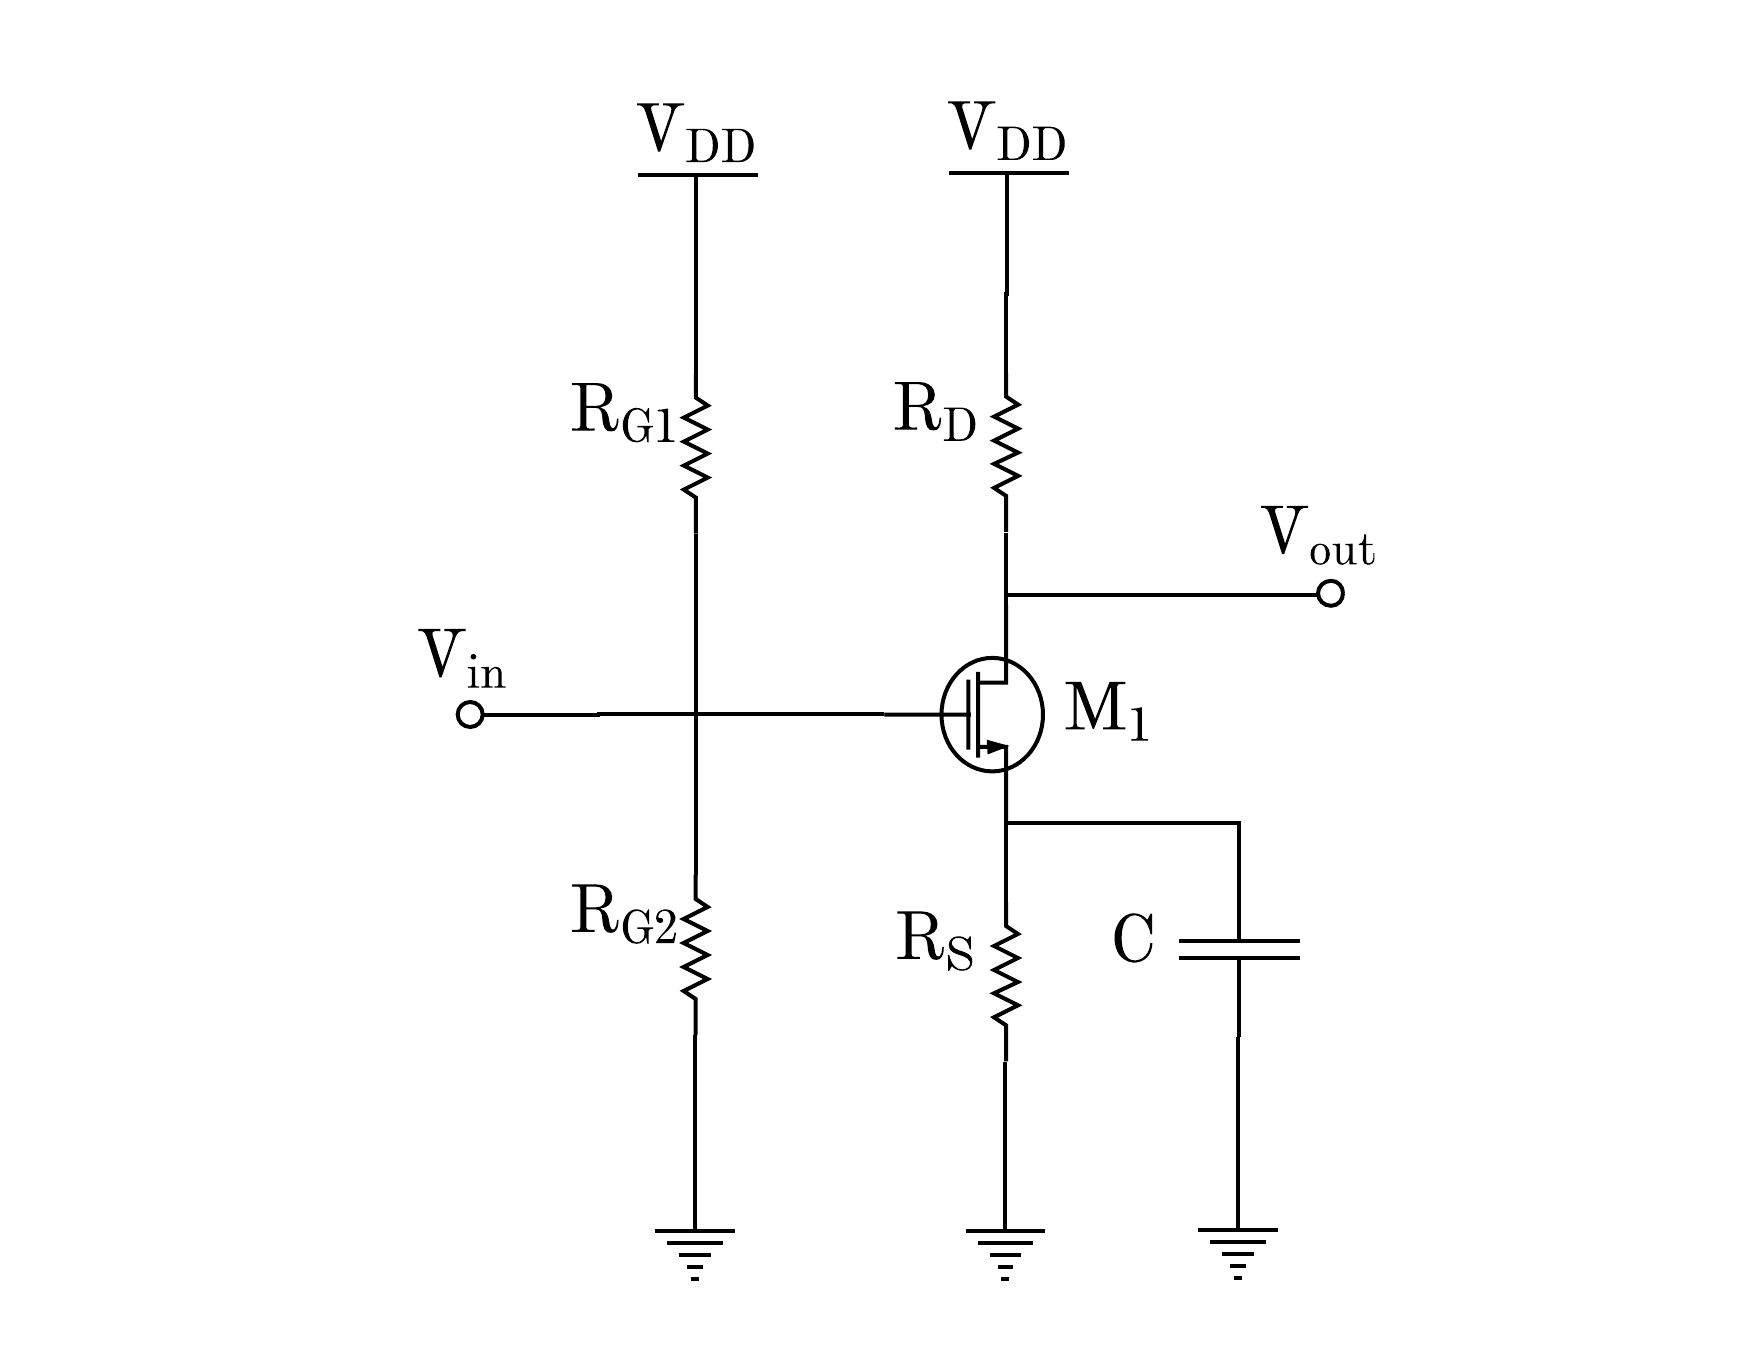
\includegraphics[width=0.75\textwidth]{second_stage}}
    \end{figure}
    As in the second stage, we choose the source voltage to be 400 mV and calculate the value of the source resistor with Ohm's law. $R_S\ \approx\ 22.4\ \Omega$. Now, we calculate the value of $V_{GS}$ using the following equation.
    $$ g_m\ =\ \frac{2I_D}{V_{GS}\ -\ V_t} $$
    $$ V_{GS}\ =\ 2.595\ V $$
    Then, the value of the gate voltage can be calculated by adding the value of the source voltage to the value of $V_{GS}$. $V_{G}\ =\ 2.995\ V$. At this point, we should verify that the transistor is operating in the saturation region. We first find the value of $V_D$ by subtracting the drop across the drain resistor from $V_{DD}$. Therefore, $V_D\ =\ 8.214\ V$. We verify that the transistor is in saturation with the following inequality.
    $$ V_{DG}\ >\ V_t $$
    $$ V_{D} - V_G\ >\ V_t $$
    $$ 8.214\ -\ 2.995\ >\ 2\ $$
    $$ 5.219\ >\ 2 $$  
    Therefore, the transistor does operate in saturation mode. \\ \\
    To obtain the values of $R_{G1}$ and $R_{G2}$, the following equation is used.
    $$ V_G\ =\ \frac{R_{G2}\ V_{DD}}{R_{G1} + R_{G2}}$$
    We set the value of $R_{G1}||R_{G2}\ =\ 1.1\ M\Omega$. Multiplying both sides by $R_{G1}$ we obtain
    $$ R_{G1}\ V_G\ =\ R_{in}\ V_{DD}$$
    $$ R_{G1}\ =\ \frac{R_{in}\ V_{DD}}{V_G}$$
    $$ R_{G1}\ =\ 3.672373\ M\Omega$$
    Using the standard equation for resistors in parallel, we find that $R_{G2}\ =\ 1.570383\ M\Omega$. \\ \\
    As stated above, the capacitor values will all initially be set to the same values. That value being $100\ \mu F$. \\  \\
   \noindent The values for the second stage are summarized below.\\ 
    \begin{itemize}
    \item $R_{G1}\ =\ 3.672373\ M\Omega$ 
    \item $R_{G2}\ =\ 1.570383\ M\Omega$
    \item $R_D\ =\ 100\ \Omega$
    \item $R_S\ =\ 22.4\ \Omega$
    \item $R_{in}\ =\ 1.1\ M\Omega$
    \item $g_m\ =\ 0.06\ \Omega^{-1}$
    \item $V_G\ =\ 2.995\ V$
    \item $V_S\ =\ 400\ mV$
    \item $V_D\ =\ 8.214\ V$
    \end{itemize}
    \subsubsection{Design of the Third Stage}
    When designing the last stage, a configuration was needed that could decrease the DC voltage level, slightly dampen the gain and have a low output impedance. The source follower with biasing provides all of these things. The $V_{GS}$ voltage drop along with the output capacitor blocks the DC voltage. The configuration also provides an AC voltage attenuation. You can see the configuration of the third stage below (Figure 4). 
    \begin{figure}[H]
        \caption{\textbf{Third Stage - Source Follower with Biasing}}
    	\centerline{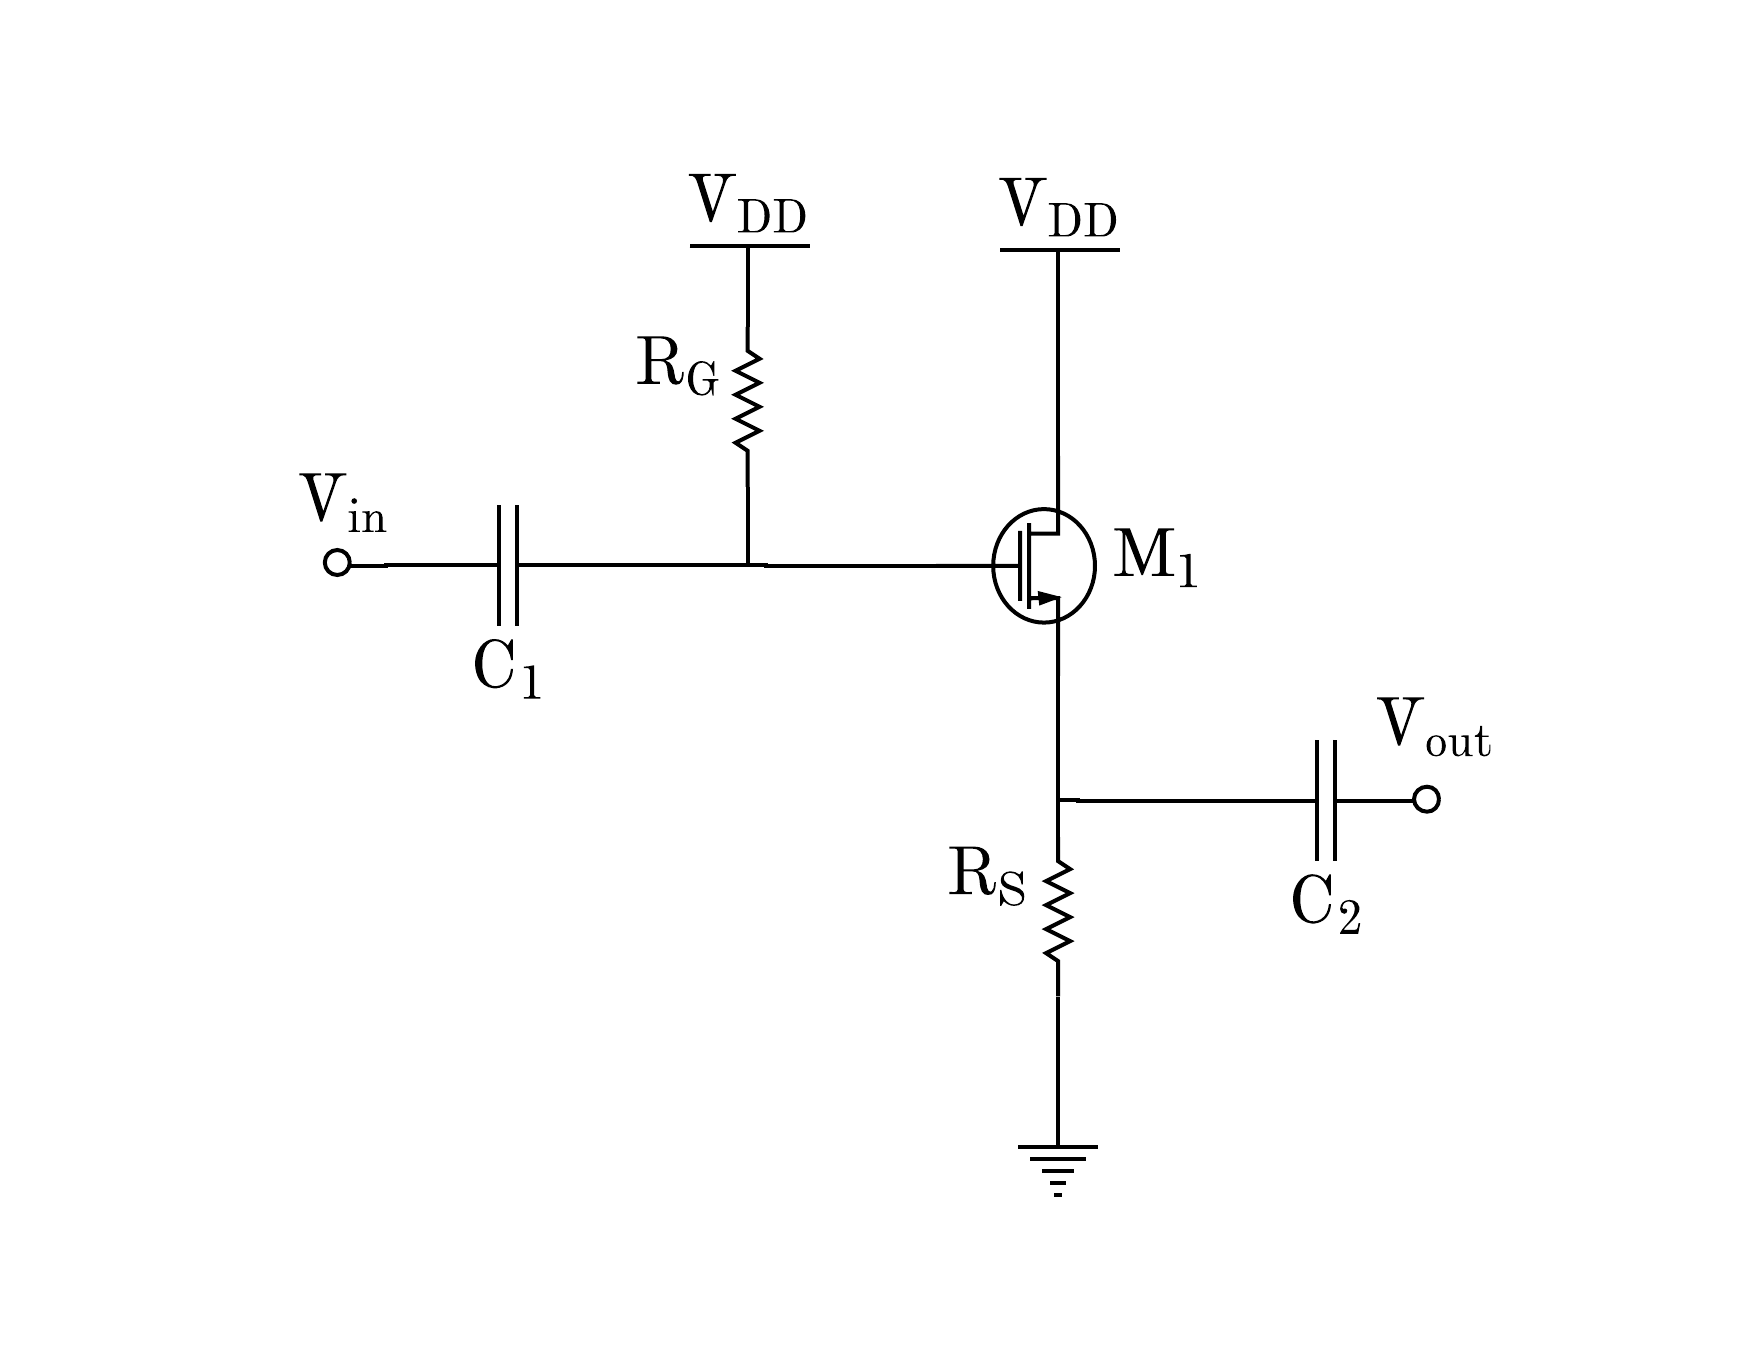
\includegraphics[width=0.75\textwidth]{third_stage}}
    \end{figure}
We choose $R_G$ to be $100\ k\Omega$ and $R_S$ to be $100\ \Omega$ to match the load resistance. Now, we need to find the output impedance of this stage since it decides the output impedance of the amplifier as a whole. The output impedance of this configuration can be found with the following equation.
$$ R_{out}\ =\ R_S||\frac{1}{g_m} $$
In order to find the value of the transconductance, the following equation is solved for $g_m$ and the known values of $A_v$ and $R_S$ are substituted.
$$ A_v\ =\ \frac{R_S}{\frac{1}{g_m}\ +\ R_S}$$ 
This yields $g_m\ =\ 0.05\ \Omega^{-1}$. Now, using the equation for $R_{out}$ above, we find that the output impedance is 16.667 $\Omega$. This is sufficiently low. 
Once again, the values of the capacitors are chosen as 100 $\mu F$.    \\
\noindent The values for the last stage are summarized below.
    \begin{itemize}
    \item $R_{G}\ =\ 100\ k\Omega$ 
    \item $R_{S}\ =\ 100\ \Omega$
    \item $R_{out}\ =\ 16.67\ \Omega$
    \item $g_m\ =\ 0.05\ \Omega^{-1}$
    \item $V_G\ =\ 10\ V$
    \item $V_S\ =\ 6.83\ V$
    \item $V_D\ =\ 10\ V$
    \end{itemize}

\subsubsection{Putting it Together}
Now that all the stages are designed, they can be combined together to get the desired behavior. Below is the final setup with decoupling capacitors and load resistance (Figure 5).
    \begin{figure}[H]
        \centerline{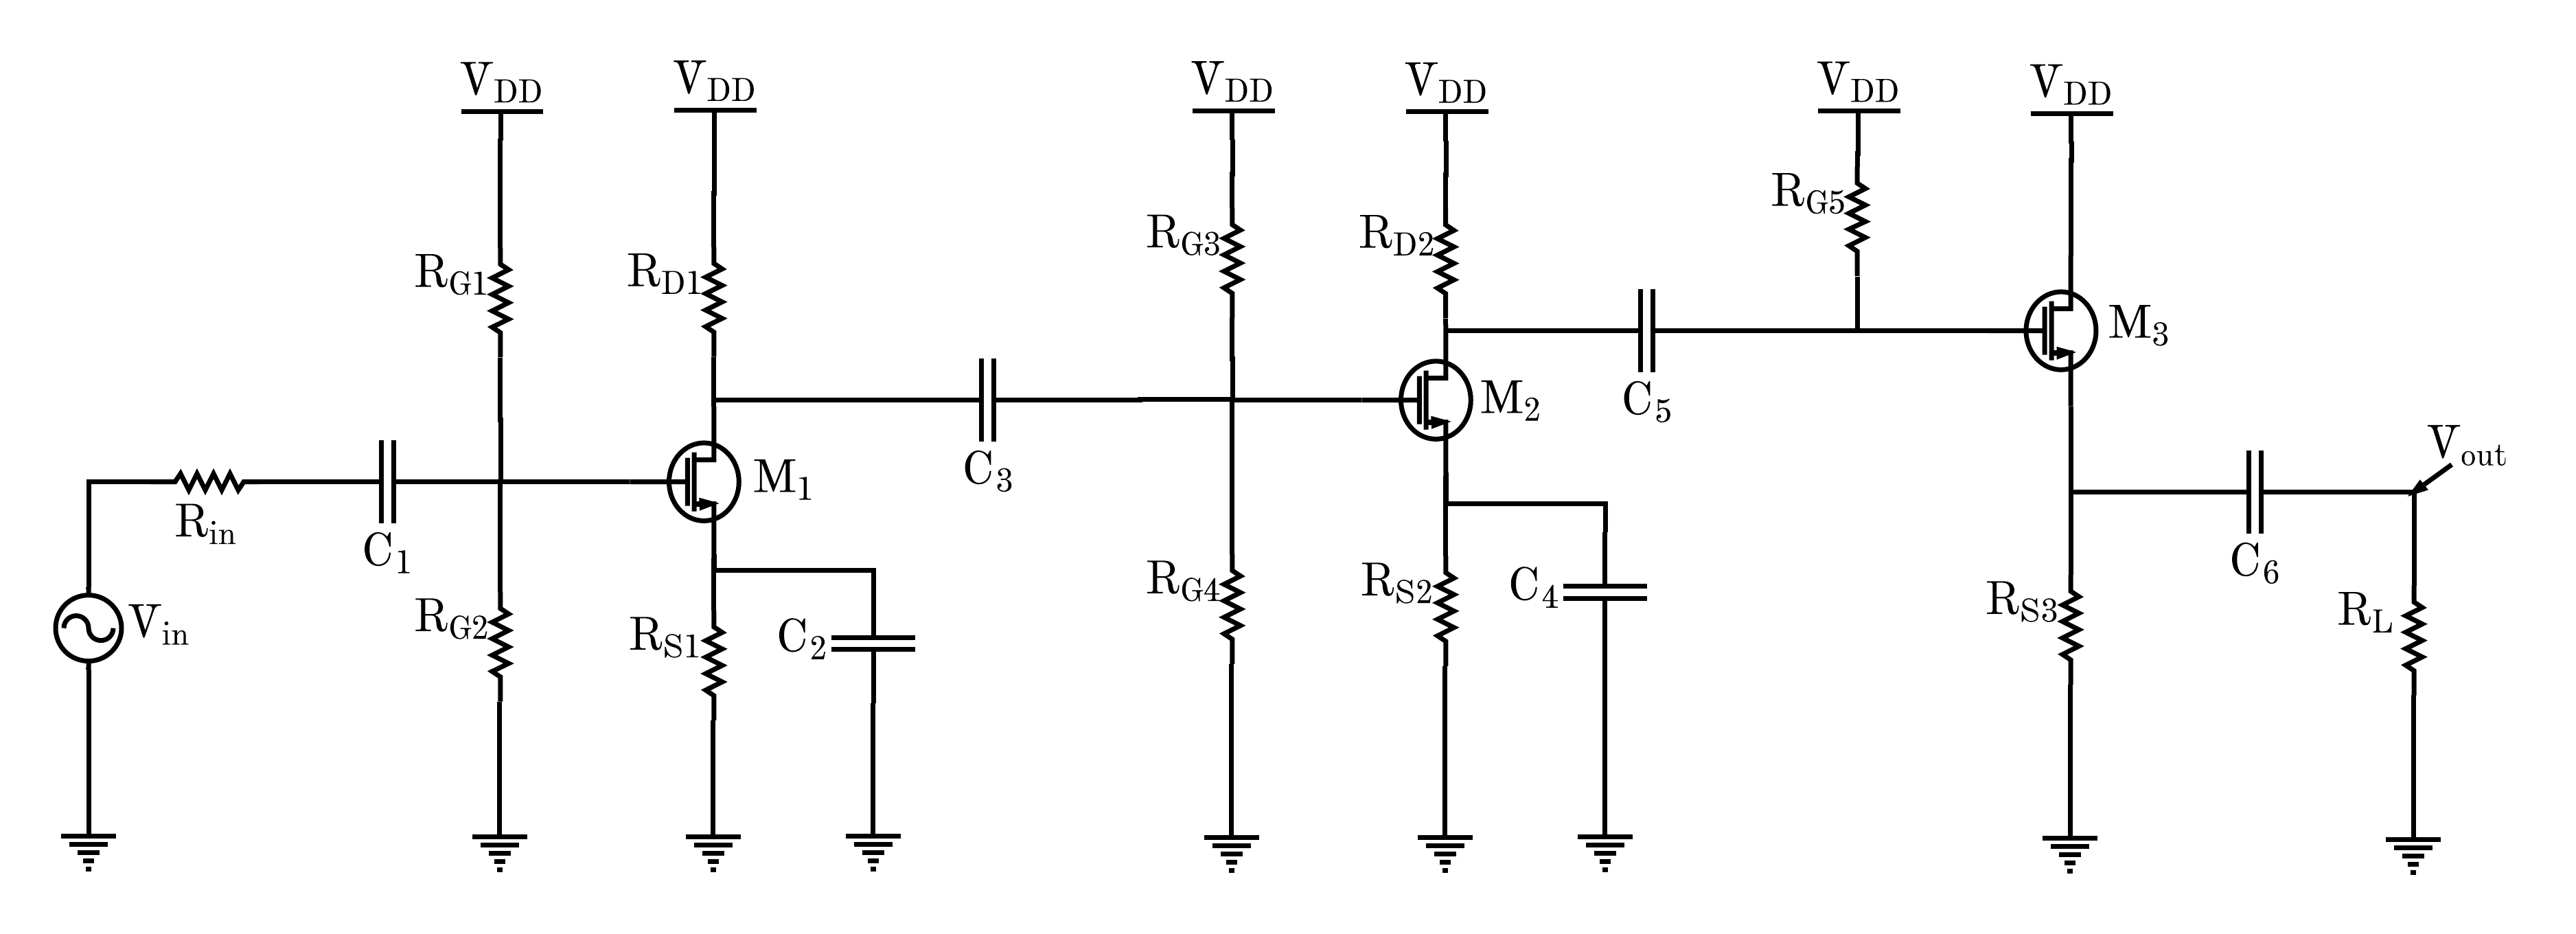
\includegraphics[width=\textwidth]{diagram}}
        \caption{\textbf{Amplifier with Decoupling Capacitors}}
	\end{figure}
   \noindent The values for the amplifier are summarized below.\\ 
    \begin{itemize}
        \item Resistors
        \begin{itemize}
        \item $R_{G1}\ =\ 15.577972\ M\Omega$ 
        \item $R_{G2}\ =\ 7.363402\ M\Omega$
        \item $R_{D1}\ =\ 100\ \Omega$
        \item $R_{S1}\ =\ 12.11\ \Omega$
        \item $R_{G3}\ =\ 3.672373\ M\Omega$ 
        \item $R_{G4}\ =\ 1.570383\ M\Omega$
        \item $R_{D2}\ =\ 100\ \Omega$
        \item $R_{S2}\ =\ 22.4\ \Omega$
        \item $R_{G5}\ =\ 100\ k\Omega$ 
        \item $R_{S3}\ =\ 100\ \Omega$
        \end{itemize}
        \item Capacitors
        \begin{itemize}
            \item $C_{1-6}\ =\ 100 \mu F$
        \end{itemize}
        \item Input Impedance = 1.1 $M\Omega$
        \item Output Impedance = 16.667 $\Omega$
    \end{itemize}
\newpage
\section{Testing}
In this section the design is verified and improved by simulating the circuit in NI Multisim.
\subsection{Biasing Verification}
The circuit was simulated with the values obtained above. The biasing points are examined to determine if our calculations were correct.
    \begin{figure}[H]
        \centerline{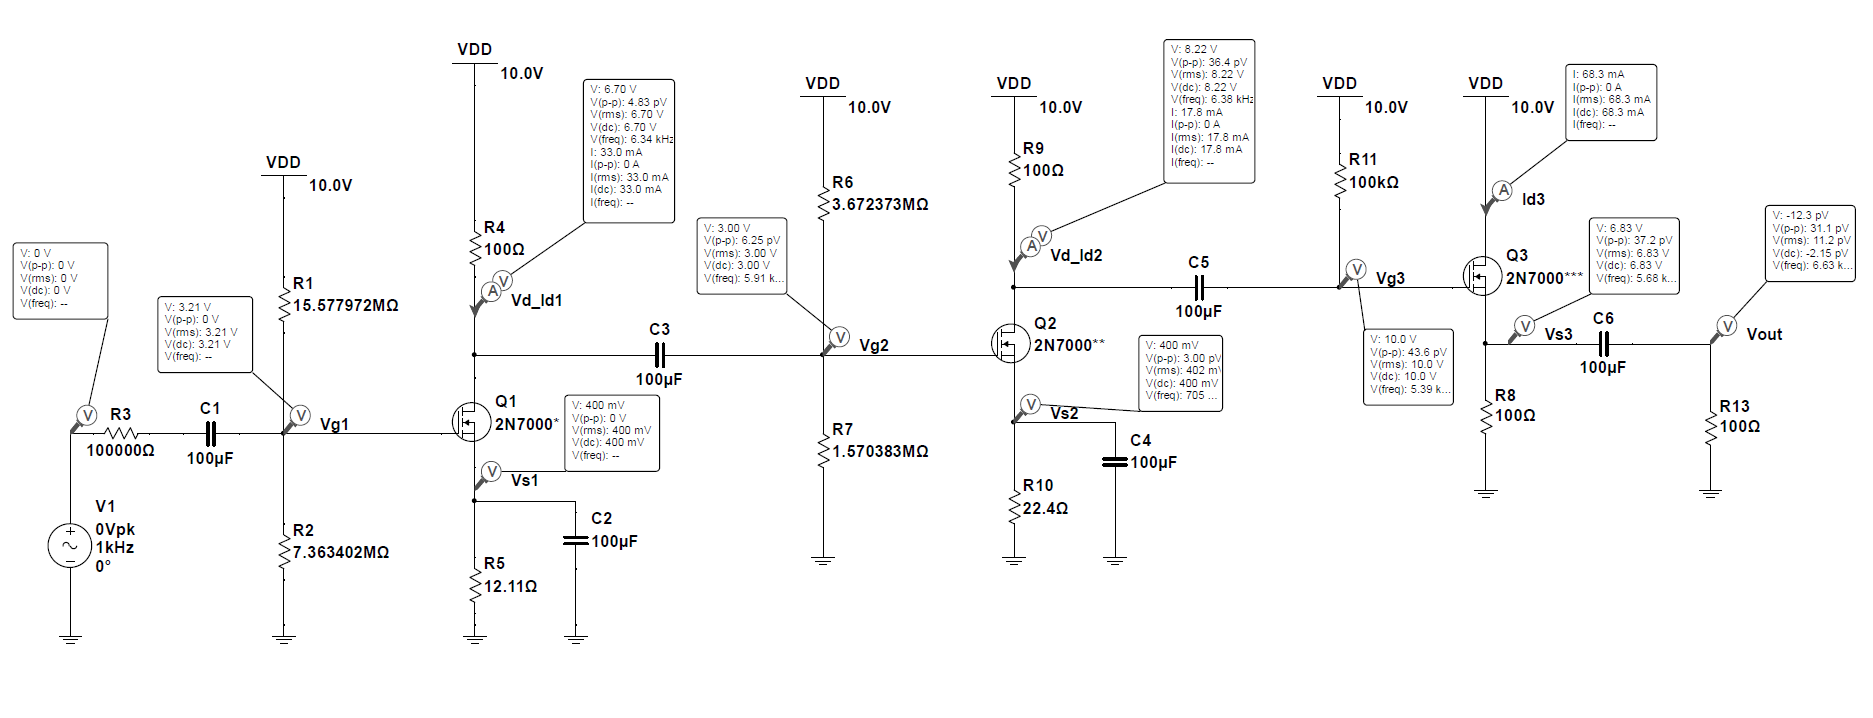
\includegraphics[width=\textwidth]{biasing_unopt_img}}
        \caption{\textbf{Biasing Points}}
	\end{figure}
In the image above, the biasing points can be seen. The values appear to be very close to the calculated values. For this reason, it is not necessary to make any changes to adjust the biasing.
\subsection{Passband Gain}
To test the passband gain a $100\ mV_{PP}$ AC sinusoidal signal was used as input to the circuit. This should result in a 4.00 $V_{PP}$ output signal. 
    \begin{figure}[H]
        \centerline{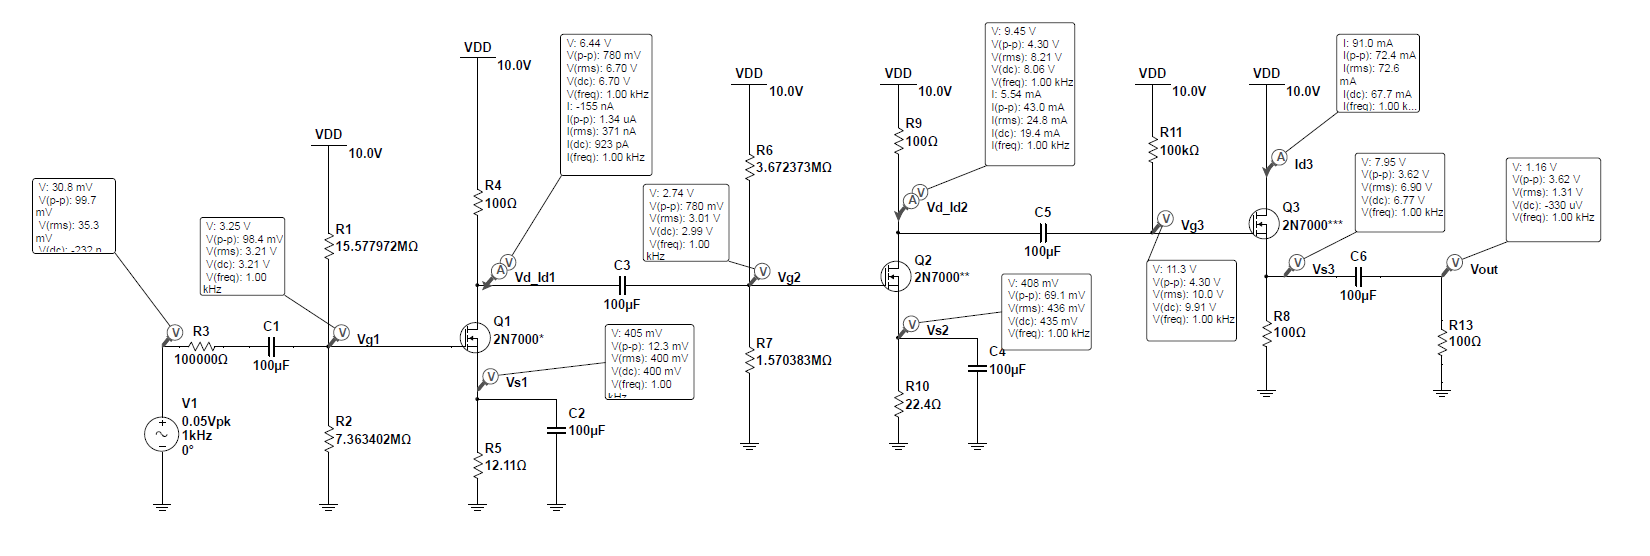
\includegraphics[width=\textwidth]{pass_band_gain_img}}
        \caption{\textbf{Passband Gain - Unoptimized}}
	\end{figure}
\subsubsection{Optimization}
Unfortunately, we do not see a gain of exactly 40 V/V. The total small signal voltage gain is approximately 36.2 V/V. The first stage is providing a gain of -7.8 V/V and second stage is providing a gain of approximately -5.5 V/V. In order to get a true 40 V/V gain, some adjustments need to be made. On the first stage, we make the following adjustment to the drain resistor. $$R_{D,new}\ =\ \frac{A_{v,desired}}{A_{v,actual}}R_{D,original}\ =\ \frac{-8}{-7.8}*100\ =\ 102.302\ \Omega$$
The same adjustment is applied to the second stage's drain resistor to obtain a value of 109.56 $\Omega$. Making this adjustment results in the first stage providing an average small signal gain of exactly -8.0 V/V and the second stage providing exactly -6.0 V/V. At the output the voltage gain is 4.02 $V_{PP}$. Which is a gain  of 40.2 V/V. These results can be seen below (Figure 8).
    \begin{figure}[H]
        \centerline{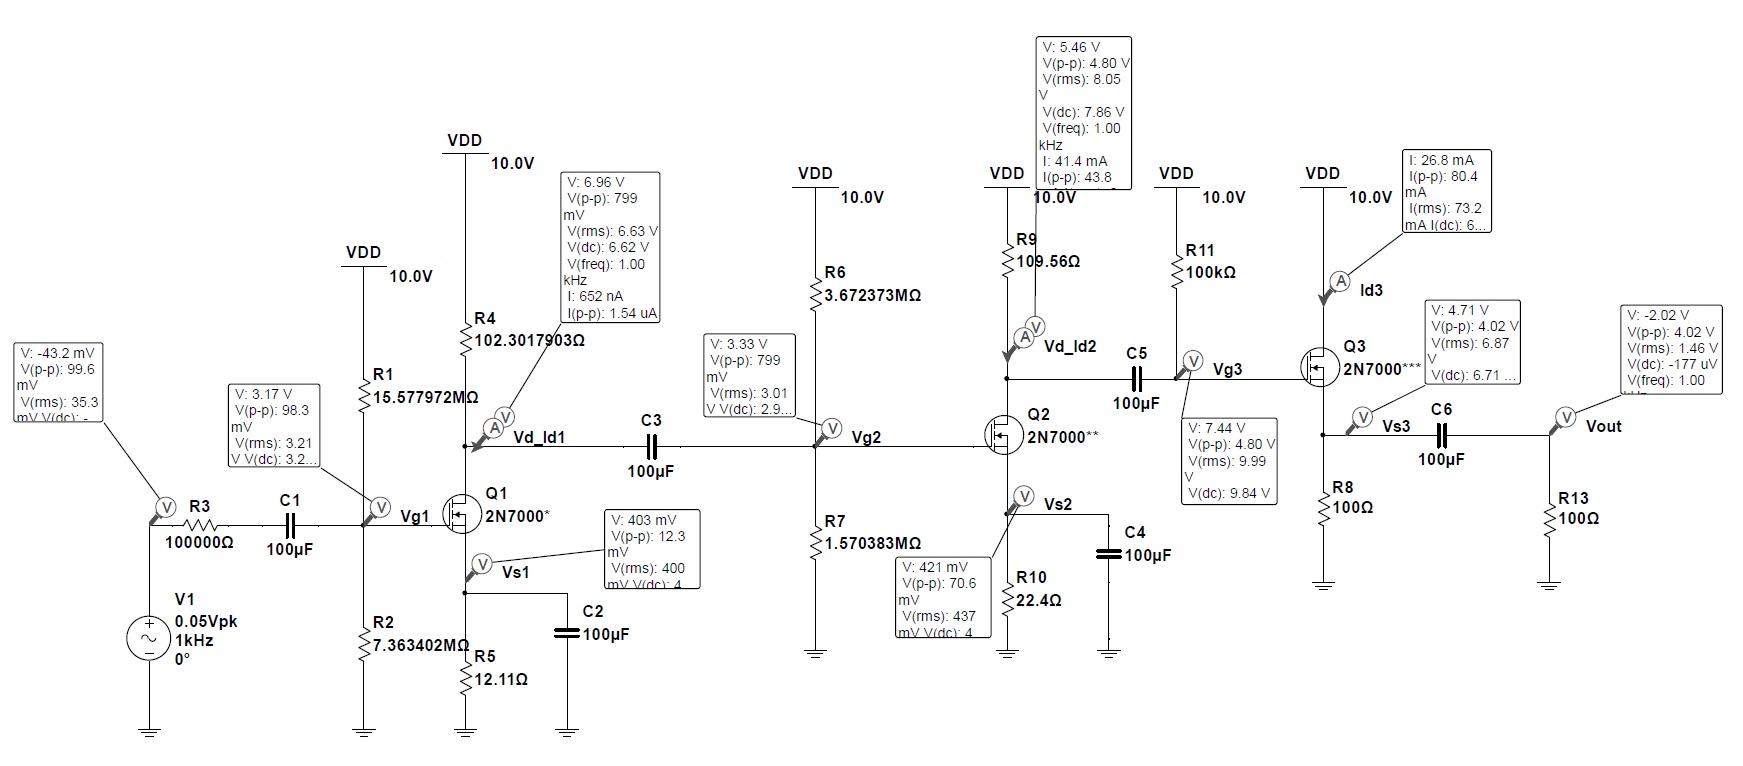
\includegraphics[width=0.95\textwidth]{pass_band_gain_opt_img}}
        \caption{\textbf{Passband Gain - Optimized}}
	\end{figure}
\subsection{Bandwidth}
In this section, the bandwidth is tested to see if the circuit's -3 dB corner frequecies occur before 50 Hz and after 20 KHz. The results of the initial testing can be seen below (Figure 9).
    \begin{figure}[H]
        \centerline{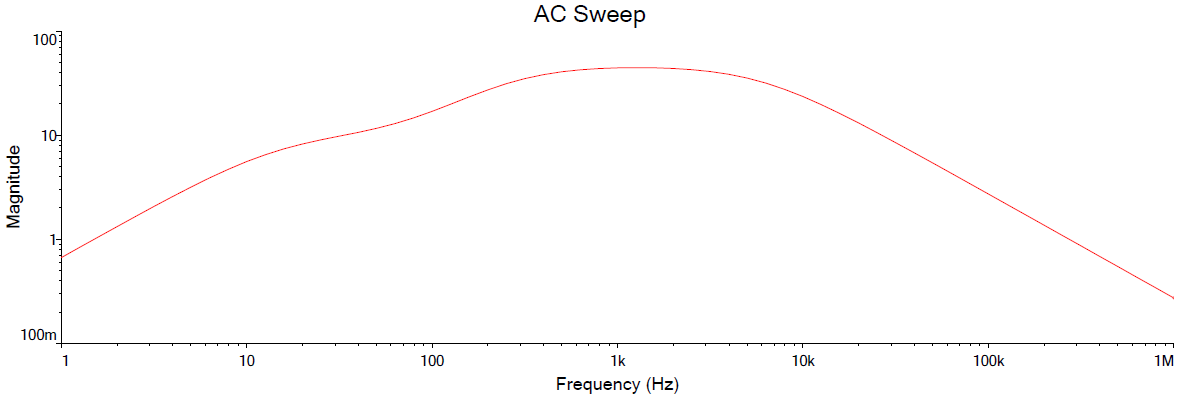
\includegraphics[width=0.9\textwidth]{bode_unopt_img}}
        \caption{\textbf{Bode Plot - Unoptimized}}
	\end{figure}
	\subsubsection{Optimization}
	It is pretty obvious that this isn't going to meet the specifications. The capacitors are causing a less than ideal bandwidth. After some experimentation, it can be observed that changing the value of the bypass capacitors attached to the source on stages one and two  can increase the bandwidth. The same is true for the decoupling capacitor attached to the output of the final stage. With this knowledge, we change the value of $C_2$ and $C_4$ from $100\ \mu F$ to 1 mF and the value of $C_6$ from $100\ \mu F$ to $90\ \mu F$. After making this modification, another AC sweep was performed. The results are below (Figure 10).
    \begin{figure}[H]
        \centerline{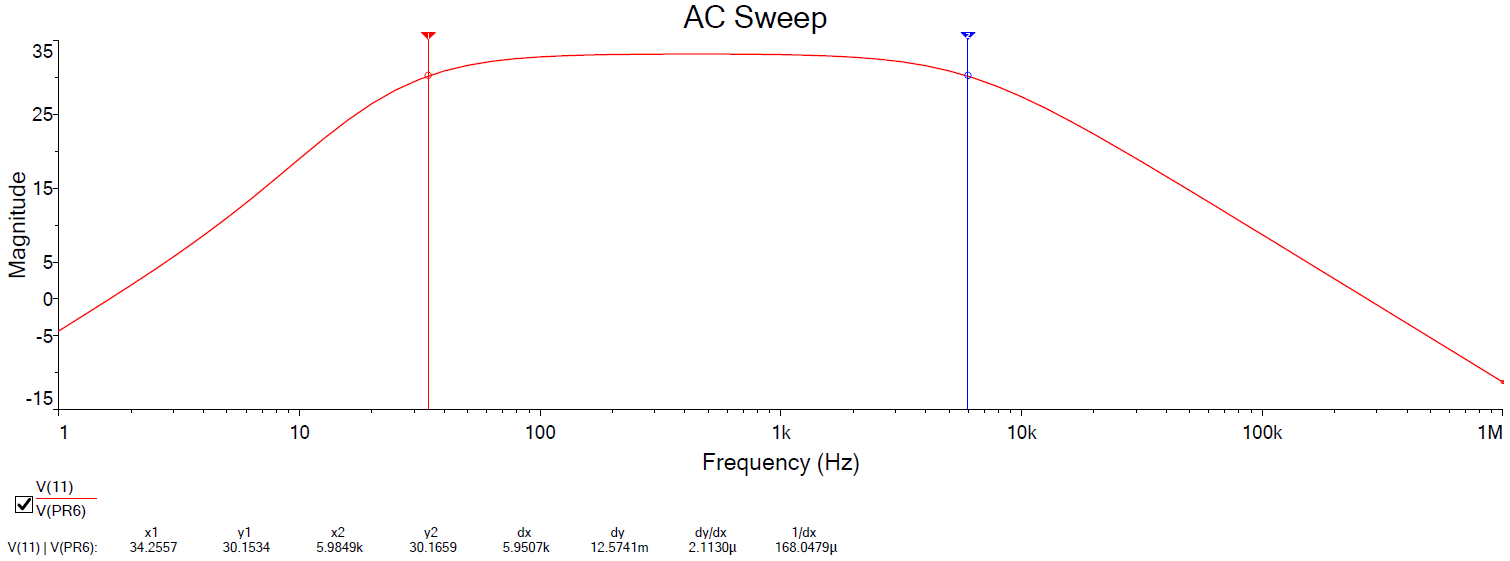
\includegraphics[width=0.85\textwidth]{bode_opt_img}}
        \caption{\textbf{Bode Plot - Optimized}}
	\end{figure}
	As you can see above, this is a marked improvement over the original. The low frequency -3 dB corner occurs at approximately 34.3 Hz and the high frequency -3 dB corner is at 5.985 kHz. Unfortunately the high frequency -3 dB corner still does not meet the specifications. The reason for this lies in the properties of the transistors themselves. The transistors have some amount of parasitic capacitance that contributes to the transfer function of the amplifier. This results in unwanted attenuation. This is something that is difficult to fix with our current level of knowledge. One problem with this modification is that it does have a minor affect on the overall voltage gain. The changes raises the small signal voltage gain from 40.2 V/V to 40.8 V/V. This change is only an increase of 1.5 \%. 
\subsection{Harmonic Distortion}
A Fourier analysis was performed in order to obtain the harmonic distortion related parameters of the amplifier. This analysis can be seen below in figures 11 and 12. 
    \begin{figure}[H]
        \centerline{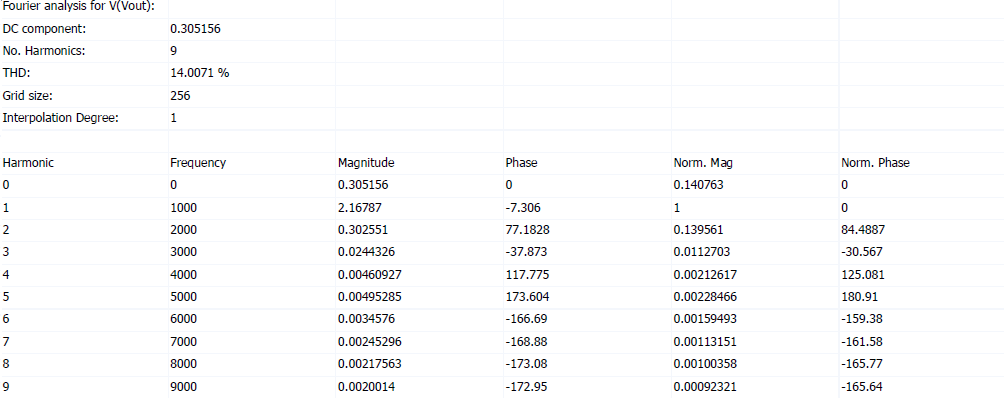
\includegraphics[width=0.75\textwidth]{distortion_chart}}
        \caption{\textbf{Distortion Analysis}}
    \end{figure}
    \begin{figure}[H]
        \caption{\textbf{Distortion Analysis Graph}}
        \centerline{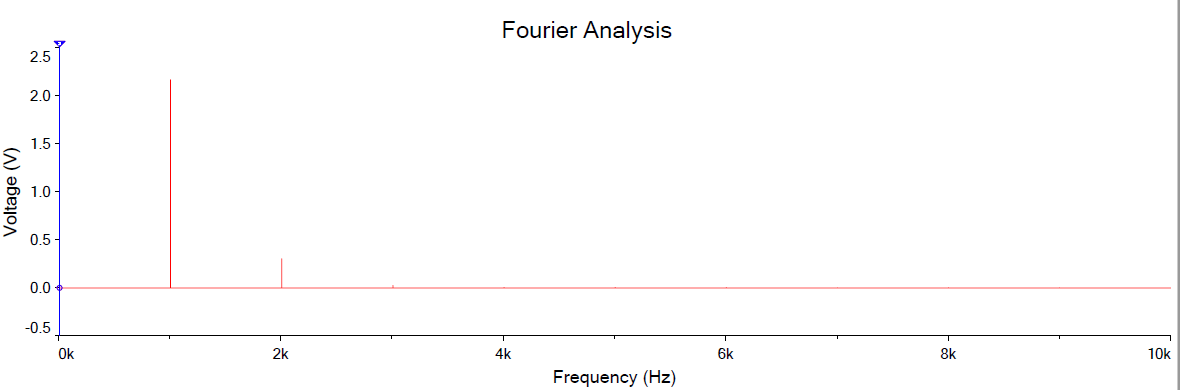
\includegraphics[width=\textwidth]{distortion_graph}}
	\end{figure}
\section{Final Circuit Design}
The final circuit design and specifications can be viewed below.
\subsection{Diagram}
\begin{figure}[H]
        \centerline{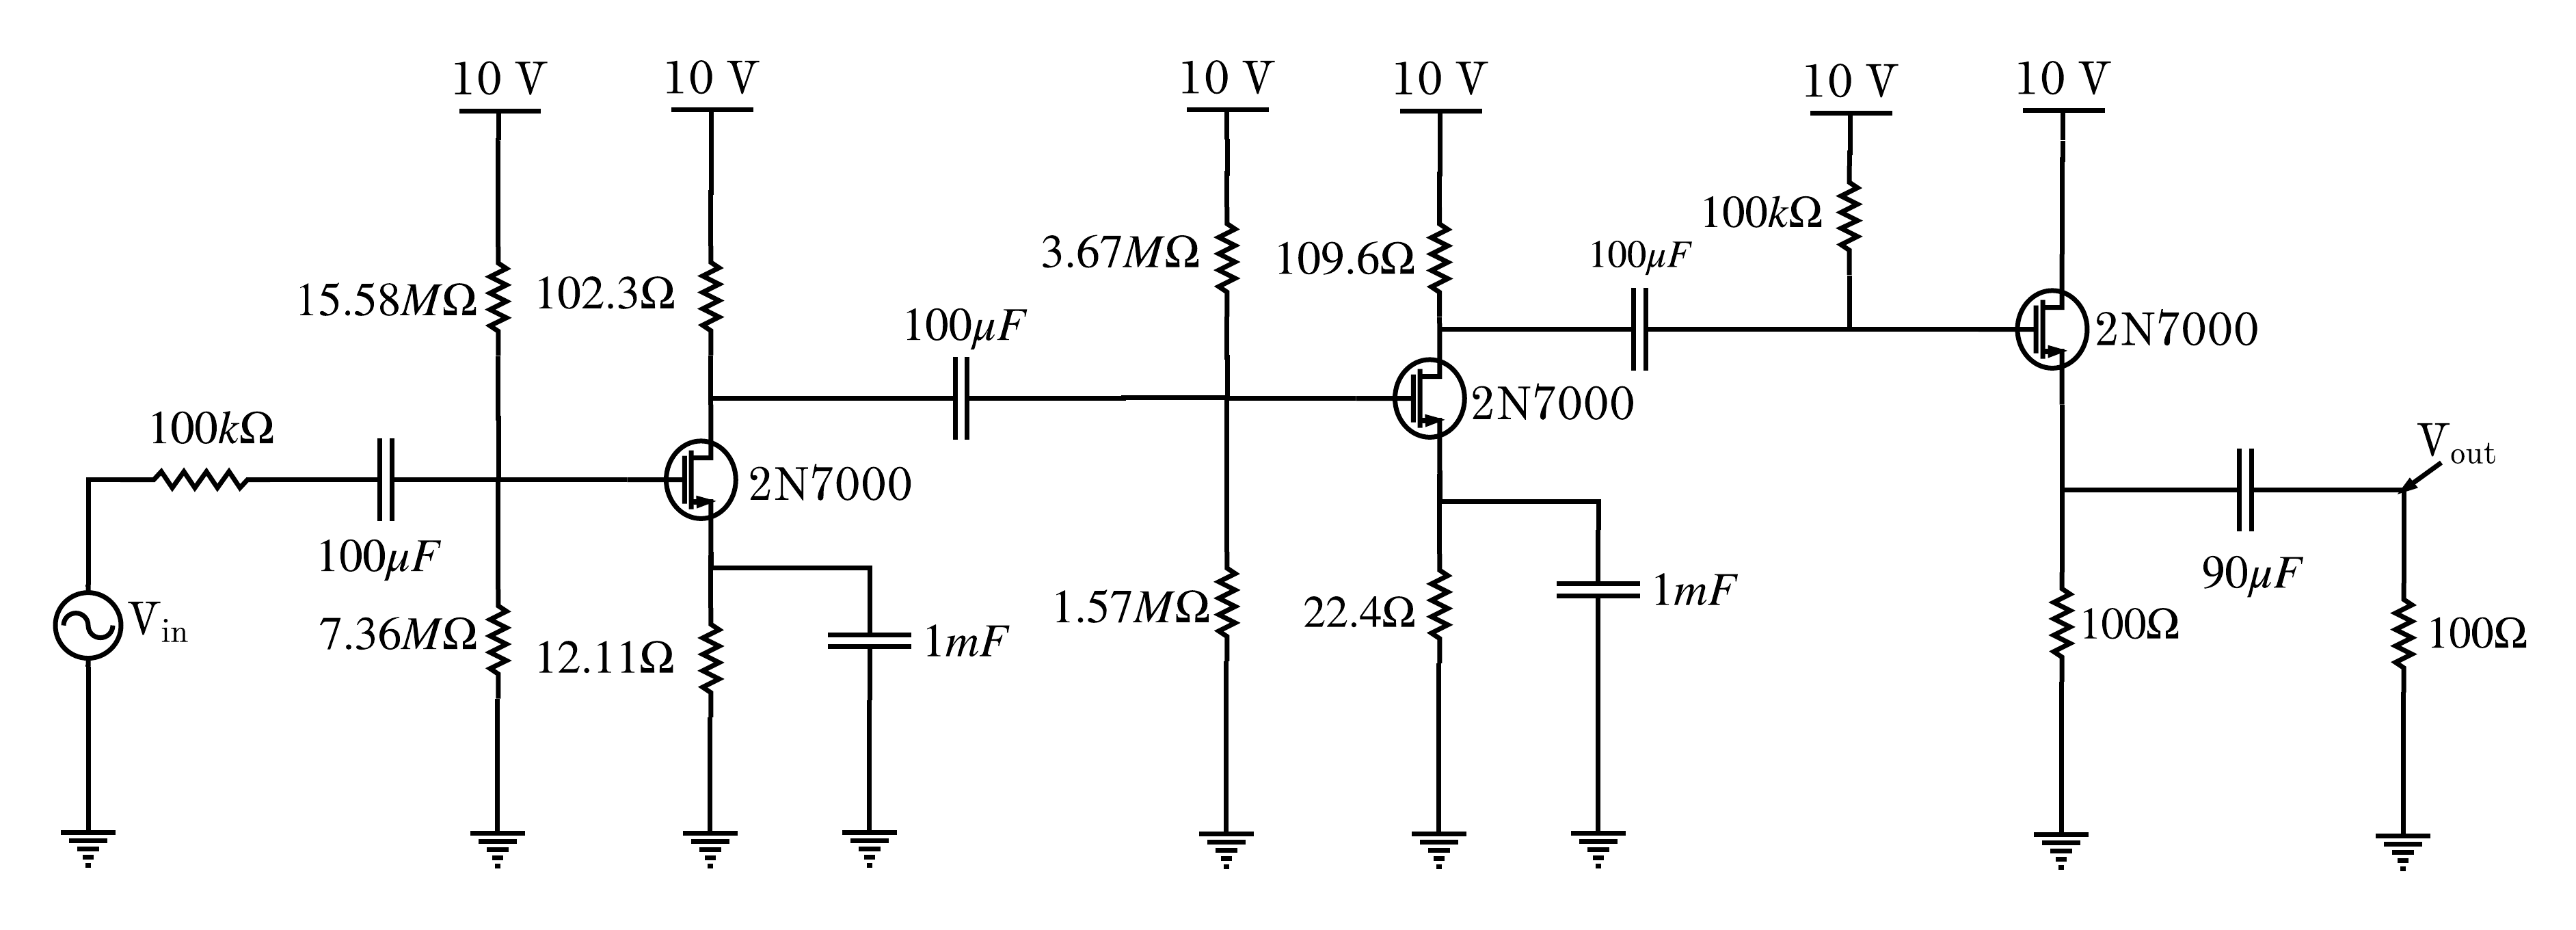
\includegraphics[width=\textwidth]{final_design}}
        \caption{\textbf{Final Design}}
	\end{figure}
\subsection{Specifications}
\begin{itemize}
    \item $A_v\ =\ 40.8\ V/V$
    \item $R_{in}\ =\ 1.1\ M\Omega$
    \item $R_{out}\ =\ 16.667\ \Omega$
    \item $Low\ Frequency\ -3\ dB\ corner\ =\ 34.3\ Hz$
    \item $High\ Frequency\ -3\ dB\ corner\ =\ 5.985\ kHz$
    \item $THD\ =\ 14\%$
\end{itemize}
\section{Conclusion}
\quad \quad This project focused on the design and classification of a CMOS amplifier. The amplifier needed to meet certain specifications. These included small signal voltage gain, input impedance, output impedance and bandwidth related specifications. First, a general topology was decided on. The decision was made to split the amplifier into three stages. Then, the individual stages were designed. Finally, the stages were combined together with decoupling capacitors. \\
\par
\quad \quad After the design phase, testing of the circuit's characteristics began. There were some slight differences between the expected values and what the simulation showed. Therefore, optimization was done to ensure the circuit met the requirements. Ultimately, the only parameter that did not meet the requirements was the high frequency -3 dB corner frequency. Unfortunately, this was due to internal parasitic capacitance of the transistors. This could be mitigated by changing the parameters of the transistors. Overall, though, the circuit gave behavior that is very close to the desired. \\
\par
\quad \quad Designing this amplifier required many (if not all) of the skills acquired in this course. Amplifier design was, at one point, one of the largest fields of study in electrical engineering. Even though this amplifier is relatively simple when compared to some others, it was incredibly interesting to get a glimpse into the process that goes into designing one of them. 

\end{document}
